\documentclass[12pt]{article}

% -- fonts (Times Roman via TeX Gyre Termes) --
\usepackage[T1]{fontenc}
\usepackage{lmodern}
\usepackage{tgtermes}

% -- layout --
\usepackage[margin=1in]{geometry}
\usepackage{setspace}
\doublespacing

% -- line numbers --
\usepackage{lineno}
\linenumbers

% -- math --
\usepackage{amsmath}

% -- tables --
\usepackage{booktabs}

% -- figures --
\usepackage{graphicx}

% -- hyperlinks (no colored links) --
\usepackage[colorlinks=false,hidelinks]{hyperref}

% -- PLOS requires "Fig" not "Figure" --
\renewcommand{\figurename}{Fig}

% ============================================================
% TITLE AND AUTHOR
% ============================================================

\title{Code Geometry, Enforcement Activation, and Exit Closure in Codified Moral Systems: An Agent-Based Model}

\author{}

\date{}

\newcommand{\affiliation}{}

\date{}

\begin{document}

\maketitle
%\noindent\affiliation
\vspace{1em}

% ============================================================
% ABSTRACT
% ============================================================

\begin{abstract}
Why do some codified moral systems sustain active enforcement while others also retain members under durable control? This paper separates two structural dimensions in an agent-based model: activation of an enforcement apparatus and members' capacity to exit. Enforcement activation follows a joint frontier in code observability and enforcement reward. With exit open, enforcement activates in many parameter cells but capture occurs in 0 of 1,890 runs. Imposed exit closure raises capture monotonically, yet cannot produce capture in a low-observability, low-reward cell where enforcement does not activate. A privilege ablation further shows that roughly 84 percent of top-five-percent punishment concentration is manufactured by institutional advantages assigned to the enforcement cadre. Finally, a diagnostic reconstruction shows that apparent endogenous closure in an earlier specification was circular because enforcer share affected both outside-option degradation and the capture criterion. The model therefore identifies distinct conditions for activation, retention, and concentration, while treating exit capacity as an exogenous structural input rather than an emergent result.
\end{abstract}
\vspace{1em}\noindent\textbf{Keywords:} agent-based modeling; institutional design; norm enforcement; organizational capture; path dependence; religious organizations

\newpage

% ============================================================
% 1. INTRODUCTION
% ============================================================

\section{Introduction}

Why are strict religious groups often unusually cohesive and durable? The canonical answer begins with religious organizations as clubs that produce collective goods. In Iannaccone's account, apparently wasteful demands can make these clubs stronger: costly requirements involving dress, diet, ritual, time, and money screen out people whose low commitment would otherwise permit them to free-ride on the sacrifices of others \citep{iannaccone1988,iannaccone1992,iannaccone1994}. Those who remain redirect resources away from competing activities and toward the group, increasing both the average commitment of members and the value of membership itself. Strictness, on this view, is not organizational pathology but a solution to adverse selection and weak participation. This club-goods framework has become the dominant economic explanation of religious strictness, as reviews of the economics of religion emphasize \citep{iyer2016,carvalho2019}. It has also generated an unusually broad family of applications. Sacrifice and nontransferable religious capital help explain ultra-Orthodox Jewish education and fertility \citep{berman2000}; monitoring institutions can sustain religious production \citep{mcbride2007}; costly signals can resolve commitment problems in religious militancy \citep{bermanlaitin2008}; and veiling can operate as a commitment device that changes social interaction and marriage-market incentives \citep{carvalho2013}. Across these applications, costly observances select committed participants and align their investments with the group.

Yet the same arrangements have another face. Every mechanism that screens at entry can simultaneously raise the cost of exit after entry. A social network concentrated inside the group is valuable to a committed member, but it is also difficult to replace after departure. An identity made inseparable from membership can deepen solidarity, but it can also make departure psychologically and socially disorganizing. Distinctive dress, diet, language, schooling, and ritual can certify commitment among insiders while isolating members from outsiders who might provide employment, friendship, marriage, or recognition. Screening and exit foreclosure are therefore the same social structure described from opposite directions. Looking inward from the organizational boundary, strictness selects and coordinates participants; looking outward from the position of a member considering departure, it degrades alternatives and makes separation costly. Case scholarship often recognizes both processes at once without analytically separating them. An analysis of the Skoptsy sect, for example, argues that high entry costs screened for devoted individuals while high exit costs reduced the viable alternatives for living outside the sect [VERIFY: citation key for the Skoptsy sect analysis]. The two mechanisms can coexist, but coexistence does not establish which one accounts for durability.

That ambiguity is now a live theoretical problem rather than a terminological distinction. \citet{bok2025} observes that research on religious exit has concentrated mainly on who leaves, why they leave, and what follows, while the forms and roles of exit costs have received comparatively little systematic theorization. The systematic theorization of the exit-cost side is therefore recent relative to the mature literature on the determinants and consequences of exit. The field has a mature screening account and a newly articulated exit-cost problem, but no design that can adjudicate their relative causal force. The identification problem is plain. In observational data, screening and exit foreclosure arrive bundled together. Any strict group that persists has already selected some people willing to bear its demands and has also organized relationships, identities, and opportunities in ways that make leaving consequential. Comparing strict and lenient groups cannot recover the separate contribution of either process, because the strictness that filters entrants also transforms the outside option of those who stay. Nor can studying former members solve the problem by itself: observed leavers are selected on having overcome the very costs whose preventive effect is at issue. Without independent variation, evidence consistent with successful screening is also consistent with blocked exit.

Agent-based simulation supplies the missing instrument because it permits the two structures to be varied as distinct inputs while measuring any coupling between their effects. An experimental design can hold the observability and rewards that support enforcement constant while changing members' capacity to leave, or hold exit conditions constant while changing whether an enforcement apparatus can activate. No observational design can cleanly impose either intervention on otherwise equivalent religious communities. The strategy follows an established computational-religion program associated with Shults and Wildman [VERIFY: publication year and citation key for Shults and Wildman], formal arguments for bringing simulation into the study of religion \citep{wildmansosis2011}, computational work linking cognition, culture, and social dynamics \citep{gorelemosshultswildman2018}, and agent-based analysis in the economics of religion \citep{iannacconemakowsky2007}. Simulation here is therefore not a substitute for historical or ethnographic evidence. It is a method for identifying structural effects that those forms of evidence necessarily observe in combination.

This paper distinguishes two structural dimensions that are largely separable, but coupled at the frontier margin: whether an enforcement apparatus activates, and whether members can leave. The quantitative caveat to this separation is reported in the results. Three findings result. First, activation follows a joint threshold in code observability and the reward for enforcement. Neither condition is sufficient alone. Across a 63-cell grid crossing nine observability levels with seven reward levels, enforcement appears along a frontier defined jointly by both parameters rather than along either axis independently. Second, exit closure is necessary but not sufficient for capture. In the exogenous closure experiment, the capture rate rises monotonically from 0 at fully open exit to 0.889 at the maximum imposed closure. Yet the low-observability, low-reward cell remains at zero capture at every closure level, including the maximum. Closing exit can retain an apparatus that activates, but it cannot create one where enforcement lacks both legibility and reward. Third, the concentration of punishment that appears to mark enforcement-dominant regimes is largely manufactured by institutional privilege. In the floor-versus-ceiling ablation, the top 5 percent of active agents issue 0.091 of punishments without the privilege bundle and 0.580 with it. Relative to the ceiling, 0.843, or roughly 84 percent, of top-5-percent concentration is privilege-manufactured. The floor Gini is 0.240, compared with 0.028 under a same-volume random-allocation null. These results distinguish the conditions that form enforcement, retain its subjects, and concentrate coercive activity. Exit capacity is treated as an exogenous structural input as a methodological safeguard. A specification in which outside-option degradation was driven by enforcer share was circular because enforcer share entered the capture criterion. Once that coupling was removed, capture occurred nowhere in the tested space, motivating the exogenous treatment used for identification.

The concentration result also qualifies a prominent interpretation in the punishment literature. The costly-punishment tradition asks how sanctioning can arise through decentralized interaction even when punishers bear private costs. Experimental and evolutionary models show how punishment can sustain cooperation and how sanctioning behavior can spread or persist under specified population and institutional conditions \citep{fehrgachter2000,boydgintisbowles2010,hauertetal2007}. From that perspective, a skewed distribution of punishment may look like an emergent product of heterogeneous strategies, repeated interaction, or selection among decentralized actors. The ablation suggests a different interpretation for delegated architectures. When one role enjoys exclusive or strongly asymmetric authority, lower costs and risks, and material reinforcement, concentrated sanctioning is substantially built into the opportunity structure before interaction generates any further inequality. This is not a general claim that punishment concentration never emerges from decentralized dynamics. It is a bounded contrast: in models with an institutionally privileged enforcement role, observed concentration cannot be treated as evidence of decentralized emergence without first removing or measuring the privileges that allocate coercive opportunities.

The mechanism is content-neutral. It is defined over structural properties: how observable a code's requirements are, what rewards attach to enforcing them, whether sanctioning authority is delegated asymmetrically, and how costly it is for a member to leave. Nothing in this definition depends on the truth, theology, or substantive moral content of a doctrine. The same logic can apply to any organization that codifies conduct and attaches status to compliance, including political movements, residential communities, firms, schools, or ideological associations. Religious regimes provide the empirical terrain because they offer the longest and richest documented record of codified conduct, costly membership, delegated moral authority, and contested exit. They also make the duality especially visible, since practices experienced as identity, discipline, and mutual commitment by some members may function as barriers to outside life for others. The paper makes no claim that codified belief tends toward coercion. Its claim is conditional and structural: where observable rules, enforcement rewards, delegated privileges, and constrained exit combine, they generate dynamics that cannot be inferred from doctrine alone.

The remainder of the paper develops the argument in four steps. The next section connects screening, exit costs, and costly punishment and derives the hypotheses. The methods section specifies the agent-based design and the independent interventions on activation, exit, and privilege. The results section presents the activation frontier, exit-closure dose-response, and privilege ablation. The conclusion states the empirical implications, limits, and tests that follow from separating selection into a group from members' capacity to leave it.

\section{Literature Positioning}

\subsection{Enforcement and strictness in the rational-choice tradition}

The dominant formal framework for understanding why high-cost religious groups persist and grow is the club-goods model developed by Iannaccone \cite{iannaccone1992,iannaccone1994}. In this framework, costly behavioral demands (dietary restrictions, dress codes, tithing, time-intensive rituals) function as screening mechanisms that exclude free-riders, raising the average quality of participation and the value of club goods (mutual aid, social capital, communal identity). Strictness is the price of admission; groups that charge higher prices attract more committed members and outcompete lenient groups in cohesion and mobilization.

This framework captures an important mechanism, and the empirical pattern it explains (that strict denominations grow while lenient ones decline) is robust. But it leaves three questions unanswered that are central to the phenomenon of enforcement-dominant dynamics. First, enforcement in the club model operates through screening (an ex ante mechanism): costly demands filter the population before entry. The model does not address ex post enforcement: the active policing, sanctioning, and punishment of members who have already joined. The transition from ``strict requirements attract committed members'' to ``enforcement specialists police the community'' is not formalized.

Second, the club model does not produce a structural distinction between moderate strictness (functional screening) and enforcement dominance (coercive control by a specialized minority). These are treated as points on a continuum rather than as qualitatively different regimes. Iannaccone \cite{iannaccone1994} acknowledged that excessive strictness can backfire: ``a church reaches [the tipping] point when it fails to offer acceptable substitutes for everything it has asked its members to give up,'' but the tipping point is not modeled as a regime transition. Third, the club model assumes voluntary participation. Members choose the strict bundle; those who dislike it leave. This assumption is reasonable for denominational choice in pluralistic religious markets but fails in contexts where exit is blocked, where apostasy carries legal penalties, kinship networks are wholly internal, or economic livelihood depends on community membership.

Berman \cite{berman2000} extended the club framework to ultra-Orthodox Jewish communities, where yeshiva attendance creates non-transferable religious human capital that functions as a powerful exit cost. Berman and Laitin \cite{berman2008} applied similar logic to terrorist organizations, where sacrifice requirements solve principal-agent problems in covert operations. Carvalho \cite{carvalho2013} formalized veiling as a commitment mechanism with implicit reputational costs for non-compliance. These extensions move closer to the dynamics of enforcement (Berman's religious capital is the strongest existing formalization of exit cost as a lock-in device), but none introduces positive enforcement payoffs to sanctioners, institutional delegation of punishment authority, or the compounding of enforcement capacity over time. The gap is consistent: the club tradition explains why strict groups can be stable but does not explain how enforcement authority concentrates in a minority or how enforcement regimes become self-reinforcing.

\subsection{Punishment, monitoring, and the observability problem}

A parallel literature in evolutionary game theory addresses the conditions under which punishment can stabilize cooperation. Boyd, Gintis, Bowles, and Richerson \cite{boyd2003} demonstrated that altruistic punishment can evolve in large groups because punishment costs decrease as punishers become common. Fehr and G\"{a}chter \cite{fehr2000,fehr2002} provided experimental evidence that costly punishment sustains cooperation and that cooperation collapses when punishment is unavailable. Axelrod \cite{axelrod1986} showed that metanorms (punishing those who fail to punish) can stabilize norm enforcement through second-order sanctioning.

These results establish that enforcement equilibria are achievable under general conditions. But a structural feature unites these models: punishment is treated as a cost to the enforcer. Punishment is altruistic; it benefits the group at the expense of the individual punisher. This is a reasonable assumption for many settings, but it does not describe the dynamics of institutionalized enforcement in codified belief systems, where enforcers routinely gain status, institutional access, and material rewards for policing. Clerical promotion contingent on orthodoxy enforcement, social prestige for public correction of deviants, and institutional budgets tied to enforcement activity all represent positive payoffs to sanctioners. When enforcement is profitable rather than costly, the dynamics change qualitatively: enforcement becomes self-sustaining not because punishers are altruistic but because the enforcement niche is structurally rewarding.

The closest formal predecessor to this dynamic is Centola, Willer, and Macy's \cite{centola2005} Emperor's Dilemma, an agent-based model where cascades of support for unpopular norms emerge when enforcement is observable and enforcers gain status. A small minority of ``true believers'' can induce majority compliance through self-reinforcing enforcement cascades. This model captures the core intuition (that enforcement can spread as a social strategy even without genuine belief), but it treats compliance as binary, does not model exit, and does not introduce institutional delegation or compounding enforcement capacity. The cascade operates through decentralized peer pressure rather than through a specialized enforcement apparatus.

A second structural limitation of the punishment literature is the treatment of observability. Punishment requires that defection (or noncompliance) be observable. This observation-dependence is implicit in nearly all punishment models but is rarely formalized as a variable property of the system being enforced. The degree to which a moral code renders compliance observable is not a constant; it is a design feature of the code itself. A code that demands observable acts (attend Friday prayers, wear prescribed clothing, observe dietary restrictions publicly) generates fundamentally different enforcement dynamics than a code that demands internal states (reduce anger, cultivate compassion, attain non-attachment). Scott \cite{scott1998} developed this insight at length for state governance (standardization and simplification render populations legible to administrative control), but no formal model has applied Scott's legibility concept to belief enforcement. This gap is the origin of our $\sigma$ parameter.

\subsection{Exit, voice, and the regime problem}

Hirschman's \cite{hirschman1970} \textit{Exit, Voice, and Loyalty} provides the canonical framework for organizational responses to decline: members can leave (exit), attempt reform (voice), or remain despite dissatisfaction (loyalty). Hirschman noted that religions explicitly position themselves as unsubstitutable, thereby raising loyalty and suppressing both exit and voice. The framework is structurally binary (exit or voice, modulated by loyalty) and does not distinguish between the qualitatively different outcomes that exit cost variation produces.

When exit is cheap and enforcement escalates, the expected outcome is fragmentation: dissatisfied members leave, the population contracts, and the enforcement apparatus loses targets. When exit is expensive and enforcement escalates, the expected outcome is very different: dissatisfied members are trapped, dissent is internalized, and enforcement can stabilize without corrective feedback from departures. These are not points on a continuum; they are distinct dynamical regimes with different attractor structures.

Kuran's \cite{kuran1995} theory of preference falsification comes closest to formalizing this distinction. Citizens publicly express preferences differing from private beliefs under social pressure, producing ``collective conservatism'' (stable falsification) or ``revolutionary cascades'' (sudden dissolution when the falsification threshold breaks). Kuran discussed religious preference falsification explicitly (crypto-Judaism under the Inquisition, Shia taqiyya) and his two-regime structure maps partially onto the collapse and mixed-enforcement regimes in our framework. However, Kuran does not formalize hierarchical capture as a distinct stable equilibrium. For him, all falsification equilibria are potentially unstable, subject to revolutionary cascade. The possibility that an enforcement-dominant minority can stabilize the system indefinitely through institutional delegation and compounding enforcement capital, preventing cascade even when private dissent is near-universal, is outside his framework.

The leaving-religion literature \cite{bromley1998,cragun2011,streib2009} provides extensive empirical documentation of exit costs and their consequences, but this scholarship is primarily descriptive and case-based. It does not formalize how exit cost interacts with enforcement parameters to generate distinct regime types. Agent-based models of secularization \cite{gelfand2011,norenzayan2013} model affiliation and disaffiliation dynamics but typically drive these through existential security or cognitive variables rather than enforcement geometry.

\subsection{Delegation, monopoly, and the missing mechanism of minority capture}

The theoretical gap that motivates this paper sits at the intersection of three well-developed literatures that have not been formally integrated.

State-formation theory provides the vocabulary of coercive monopoly. Weber \cite{weber1946} defined the state by its successful claim to monopoly over legitimate force. Tilly \cite{tilly1985} described state-making as organized coercion with a ratcheting dynamic: war requires taxation, taxation requires administrative capacity, administrative capacity enables more war. Mann \cite{mann1986} distinguished despotic power (command) from infrastructural power (the capacity to penetrate society with rules and monitoring). These frameworks describe compounding coercive capacity at the macro-political level but have rarely been applied to the internal governance of belief systems.

New institutionalism provides the theory of enforcement equilibria and path dependence. North \cite{north1990} defined institutions as formal and informal constraints plus enforcement characteristics, and noted that ``formal rules are created to serve the interests of those with the bargaining power to create new rules'': minority capture by institutional design. Greif \cite{greif2006} analyzed the transition from distributed to specialized enforcement in merchant communities. Greif and Mokyr \cite{greif2016} observed that ``the fact that such an agent has been asked to legitimize a ruler is a source of additional power to such agents,'' a description of compounding enforcement capital that remains unformal. Pierson \cite{pierson2000} formalized path dependence as an increasing-returns dynamic where early institutional advantages compound over time.

Political economy of religion provides case studies of enforcement delegation. Rubin \cite{rubin2017} analyzed religious authorities as ``legitimizing agents'' who sit at the political bargaining table; Ottoman ulama monopolized religious scholarship and commercial law interpretation for centuries. Cook \cite{cook2000} traced the Islamic hisbah doctrine from individual Muslim obligation to institutional enforcement apparatus. Given \cite{given1997} documented how the medieval Inquisition accumulated records, informers, and procedural knowledge that compounded its enforcement capability across decades. Kelly \cite{kelly1989} described the transition from personal inquisitorial authority to institutional jurisdiction, the shift from distributed to delegated enforcement.

Each of these literatures contains ingredients of the mechanism we formalize: coercive monopoly, enforcement delegation, compounding capacity, path dependence. But they have not been combined into a unified micro-level model that derives enforcement regimes from the interaction of code structure and institutional design. Evolutionary game theory has partially filled this gap through the distinction between peer punishment and pool punishment \cite{hilbe2014,sigmund2010}, showing that delegated institutional punishment produces qualitatively different equilibria than distributed individual punishment. But pool-punishment models treat the institution as solving the second-order punishment problem (who punishes non-punishers?), not as enabling minority capture of doctrinal authority through compounding enforcement capital.

\subsection{The gap}

No existing formal model combines the following five components: (1) legibility of moral compliance as a continuous structural parameter of the code, distinct from signaling cost; (2) positive enforcement payoffs to sanctioners, generating a self-sustaining enforcement niche; (3) exit cost as a regime determinant that distinguishes collapse from capture; (4) institutional delegation of punishment authority, concentrating enforcement in a minority; and (5) compounding enforcement capital that creates path-dependent power accumulation in the enforcement apparatus.

Each component has strong antecedents. Iannaccone formalized costly demands; Boyd et al.\ formalized punishment dynamics; Berman formalized exit costs; Weber \cite{weber1946} and Tilly \cite{tilly1985} described coercive monopoly; Greif and Pierson described path dependence. Their synthesis permits the model to separate enforcement activation from retention, test how institutional privilege allocates punishment, and distinguish continuous outcomes from researcher-defined regime classes.

The contribution of this paper is to build that synthesis as a working computational model, demonstrate its regime structure, identify the causal mechanism through ablation, and provide a falsifiable scoring rubric for empirical evaluation.


% ============================================================
% 3. THEORETICAL FRAMEWORK
% ============================================================

\section{Theoretical Framework}

\subsection{Codified Moral Systems}

A codified moral system is a socially shared normative structure in which obligations, prohibitions, and membership criteria are articulated in transmissible rule-form and maintained across generations through institutional mechanisms. Religious traditions are the most historically durable instances. The framework developed here is not restricted to religion; any identity-bearing system that codifies behavioral expectations and enforces compliance falls within scope. Political ideologies with loyalty tests, revolutionary movements with purity requirements, and professional bodies with ethical codes all instantiate codification to varying degrees.

As codified systems scale beyond face-to-face interaction, they confront a structural problem: moral quality must be made legible. Internal states (intention, sincerity, compassion, detachment) are opaque to observers. Institutions that must evaluate adherence therefore face pressure to adopt observable proxies. Ritual participation, dress codes, dietary restrictions, speech markers, formal declarations, and codified behaviors become instruments of classification. This shift is not incidental. It is a functional response to the problem of monitoring at scale. But it alters the incentive structure of the system. When moral standing becomes externally classifiable, enforcement roles become structurally viable.

We formalize this transformation as a problem of code geometry: the structural configuration of a codified moral system along dimensions that jointly determine whether enforcement equilibria become reachable.

\subsection{Dimensions of Code Geometry}

Five structural dimensions characterize the enforcement landscape of a codified system. These are not evaluative. They describe the formal properties of the code, not the moral worth of any tradition.

\textbf{Legibility ($\sigma$)} refers to the degree to which compliance can be externally observed and socially verified. A system is highly legible when observers can classify adherence through visible acts (dress, attendance, dietary practice, ritual performance, verbal formulae) without privileged access to internal states. A system is low in legibility when compliance depends on dispositions that cannot be reliably assessed by third parties. Legibility determines the feasibility of monitoring.

\textbf{Substitutability} captures whether externally observable compliance can function as a sufficient condition for moral standing. In high-substitutability systems, ritual performance or formal adherence terminates moral evaluation: an agent who fulfills the visible requirements is classified as moral regardless of internal state. In low-substitutability systems, external acts are explicitly necessary but insufficient; moral status depends on interior transformation that cannot be replaced by proxy performance.

Substitutability is analytically distinct from legibility. A system may render compliance visible (high legibility) without allowing visible compliance to substitute for interior reform (low substitutability). The joint condition (high legibility and high substitutability) is what makes proxy compliance a stable strategy: agents can achieve moral standing through externally performable acts alone, and observers accept this.

In the agent-based model, the parameter $\sigma$ represents the joint legibility-substitutability axis. Formally, $\sigma$ is the weight of external compliance ($s_i$) relative to internal cultivation ($x_i$) in the perceived moral score: $m_i = (1 - \sigma)x_i + \sigma s_i$. At low $\sigma$, moral evaluation depends on internal states that are opaque to observers; monitoring is infeasible and enforcement is unrewarding. At high $\sigma$, moral evaluation terminates at visible performance; monitoring is cheap and enforcement becomes structurally viable. The model collapses legibility and substitutability into a single parameter because in most codified systems these covary: systems that make compliance externally visible also tend to accept visible compliance as sufficient for moral standing. The theoretical framework distinguishes them because they can separate (monastic behavioral codes, for instance, render compliance visible without treating external observance as sufficient for spiritual attainment). The model tests the joint condition because it is the joint condition that creates the enforcement niche. Concrete indicators of high-$\sigma$ systems include dress-code compliance, attendance records, dietary markers, public prayer performance, and verbal orthodoxy tests. Concrete indicators of low-$\sigma$ systems include meditative attainment stages, sincerity of intention, character transformation, and contemplative depth. The separate observability parameters ($v_{\text{obs}}$, $a_{\text{obs}}$) in the model handle the pure observation-accuracy dimension: $v_{\text{obs}}$ captures how reliably external compliance signals are perceived, while $a_{\text{obs}}$ captures the (typically very low) probability that internal states are observable.

\textbf{Enforcement affordance} refers to the ease with which deviations can be detected, classified, and sanctioned. Systems with binary violation categories (permitted/forbidden), well-defined infraction types, and established institutional sanction pathways possess high enforcement affordance. Systems characterized by interpretive ambiguity, graduated evaluation, and contested authority possess low enforcement affordance. High enforcement affordance reduces the per-act cost of policing.

\textbf{Centralization of adjudication} describes whether interpretive and disciplinary authority is monopolized or distributed. Under high centralization, a recognized clerical, judicial, or institutional body defines orthodoxy, controls appeals, and limits interpretive plurality. Under low centralization, multiple legitimate interpretive authorities coexist, norm enforcement is local and heterogeneous, and no single body can authoritatively define deviation. Centralization does not itself produce enforcement, but it amplifies enforcement once initiated by coordinating sanctioning across a population.

\textbf{Exit cost} refers to the social, economic, legal, and identity penalties associated with leaving or dissenting from the system. When exit cost is high (apostasy carries severe sanctions, kinship networks are internal to the community, economic livelihood depends on membership, identity foreclosure makes departure psychologically costly), disaffected members are trapped. Dissent is expressed internally rather than through departure. When exit cost is low, enforcement escalation produces fragmentation rather than compliance: members leave rather than submit. Exit cost therefore determines whether tightening leads to collapse or persistence.

\subsection{From Geometry to Regimes}

The interaction of these dimensions generates distinct structural regimes. Four are consistently observed in simulation and have historical correlates.

In the \textit{quiet regime}, legibility and enforcement affordance are low, or enforcement reward is insufficient to sustain sanctioning as an adaptive strategy. Punishment remains negligible, exit is low, and the system persists without generating an enforcement niche. The code may be codified, but its structure does not render compliance auditable or sanctioning profitable.

In the \textit{collapse regime}, legibility and enforcement affordance are high but exit cost is low. Enforcement escalation triggers departure. The population shrinks, monitoring loses targets, and the system fragments. Tightening is self-defeating.

In the \textit{capture regime}, legibility, substitutability, and enforcement affordance are jointly high and exit cost is also high. Enforcement escalation does not produce mass departure. Sanctioning stabilizes because it is rewarded: enforcers gain status, institutional access, or material benefits. Compliance becomes self-reinforcing. The system converges on an enforcement-dominated equilibrium in which visible compliance is near-universal but may coexist with private dissent.

In the \textit{mixed regime}, exit is feasible but non-trivial, and membership confers benefits sufficient to retain a substantial fraction of the population. Partial exit coexists with a hardened enforcement core. Overall prevalence may decline, but active participants exhibit higher rigidity and enforcement intensity than the pre-tightening population. The system persists in reduced form.

These regimes arise from structural incentives. They do not require abnormal psychological distributions, charismatic leaders, or exogenous political shocks, though all of these can shift parameters and change which regime the system occupies.


% ============================================================
% 4. PARAMETER-OBSERVABLE MAPPING
% ============================================================

\section{Parameter-Observable Mapping}

The agent-based model is intended not as an abstract toy, but as a formalization of observable structural features of codified moral systems. Each model parameter corresponds to a property that can, at least in principle, be identified in historically bounded institutional settings without taking a theological position on the truth or falsity of the underlying doctrine. The aim of this section is therefore not to rank traditions, but to specify how a regime can be located in a common structural space.

\subsection{Parameter-to-observable mapping}

The mapping proceeds from model parameters to institutional indicators. Legibility refers to the extent to which compliance is externally classifiable through visible acts, speech, dress, attendance, dietary practice, or other public markers. Empirically, this dimension is approximated by the proportion of canonical prescriptions and disciplinary expectations that target observable behavior rather than opaque interior states. Substitutability refers to whether such visible compliance is treated as sufficient, or near-sufficient, for moral standing. A regime scores high on substitutability when external performance functions not merely as evidence of discipline, but as an accepted proxy for virtue, orthodoxy, or salvation.

Enforcement affordance refers to the ease with which deviations can be detected, coded as violations, and linked to sanctions. Observable indicators include the presence of binary or low-ambiguity rule structures, explicit violation categories, routinized complaint channels, and established disciplinary procedures. Centralization refers to the concentration of interpretive and punitive authority. It is indexed by the existence of recognized adjudicating bodies, monopoly claims over orthodoxy, restricted appeal channels, and institutional mechanisms that convert local accusations into system-wide disciplinary action. Exit cost refers to the penalties associated with leaving, defecting, or openly dissenting. It is approximated by legal apostasy penalties, kinship endogamy, economic dependence on the community, identity foreclosure, and the social cost of disaffiliation.

The model also includes enforcement reward and delegation variables, which are especially important for distinguishing mere rule density from enforcement specialization. Enforcement reward is operationalized through promotion incentives, prestige for orthodoxy policing, access to institutional resources, or material compensation tied to disciplinary activity. Delegation is operationalized through the existence of specialized offices, enforcement jurisdictions, or recognized actors whose role includes monitoring and sanctioning others. The complete scoring anchors and observable proxies are provided in Online Resource 1; the purpose of the present section is to make explicit the logic of the mapping rather than duplicate the full rubric.

% -- Tables 1-4: Parameter-to-observable mapping --

\begin{table}[ht]
\centering
\caption{Code geometry dimensions and observable indicators.}
\label{tab:dimensions}
\begin{tabular}{lp{5.5cm}p{5.5cm}}
\toprule
Dimension & Model parameter & Observable indicators \\
\midrule
Legibility & $\sigma$ (substitution weight, 0--1) & Proportion of prescriptions targeting visible behavior; dress codes, attendance records, dietary markers \\
Substitutability & Collapsed into $\sigma$ & Whether visible compliance is accepted as sufficient for moral standing \\
Enforcement affordance & $\pi$ (enforcement reward), $\kappa$ (cost) & Binary violation categories, routinized complaint channels, established sanction pathways \\
Centralization & Cadre selection, monopoly flag & Recognized adjudicating bodies, monopoly over orthodoxy, restricted appeals \\
Exit cost & base\_opp, $\delta$, exit\_threshold & Legal apostasy penalties, kinship endogamy, economic dependence, identity foreclosure \\
\bottomrule
\end{tabular}
\end{table}

\begin{table}[ht]
\centering
\caption{Agent-level parameters and defaults.}
\label{tab:agent-params}
\begin{tabular}{llll}
\toprule
Parameter & Symbol & Default & Description \\
\midrule
Legibility weight & $\sigma$ & 0.75 & Weight of external compliance in moral perception \\
External observability & $v_{\text{obs}}$ & 0.90 & Probability of observing external compliance \\
Internal observability & $a_{\text{obs}}$ & 0.05 & Probability of observing internal cultivation \\
Enforcement reward & $\pi$ & 0.22 & Status gain per successful punishment \\
Enforcement cost & $\kappa$ & 0.08 & Backlash risk per punishment act \\
Punishment severity & $\lambda$ & 0.25 & Utility penalty imposed on target \\
Literalism trait & $L$ & Beta(1.5, 4.5) & Fixed agent trait, right-skewed \\
\bottomrule
\end{tabular}
\end{table}

\begin{table}[ht]
\centering
\caption{Institutional and network parameters.}
\label{tab:inst-params}
\begin{tabular}{llll}
\toprule
Parameter & Default & Range tested & Function \\
\midrule
Population $N$ & 350 & Fixed & Agent count \\
Network & Scale-free & Fixed & Barab\'asi--Albert \\
Enforcer quota $q$ & 0.08 & 0.04--0.25 & Fraction designated as cadre \\
Authority threshold & 0.35 & Fixed & $A$ level activating monopoly \\
Capital gain/punish & 0.15 & Fixed & Compounding per act \\
Capital decay & 0.005/step & Fixed & Slow institutional decay \\
Shock schedule & $t = 100, 220, 320$ & Fixed & Exogenous threat timing \\
\bottomrule
\end{tabular}
\end{table}

\begin{table}[ht]
\centering
\caption{Exit and retention parameters.}
\label{tab:exit-params}
\begin{tabular}{llll}
\toprule
Parameter & Default & Range tested & Function \\
\midrule
Base opportunity & 0.30 & 0.30--0.90 & Baseline outside-option quality \\
Exit threshold & $-1.0$ & $-1.0$, $1.5$ & Utility level triggering exit evaluation \\
Block exponent & 2.5 & Fixed & Nonlinear exit suppression \\
Exit cost & 0.4 & Fixed & Per-departure penalty \\
Alt. degradation $\delta$ & 0.0 & 0.0--1.0 & Perceived outside-world quality \\
Drift speed $\eta$ & 0.0 & 0.0--0.30 & Rate of endogenous $\delta$ drift \\
Punish floor & 0.08 & 0.04--0.15 & Intensity gate for drift activation \\
\bottomrule
\end{tabular}
\end{table}

\subsection{What this mapping does and does not claim}

This mapping does not claim that any single dimension is sufficient to determine regime type. The theory is configurational. High legibility without high exit cost may generate fragmentation rather than capture. High exit cost without legibility may trap members without producing a stable enforcement niche. High centralization without substitutability may concentrate adjudication while still failing to make visible compliance a dominant strategy. The predictive object is therefore the joint geometry of the regime, not an isolated score.

The mapping also does not treat traditions as fixed wholes. The unit of analysis is a historically bounded regime in a specific institutional and legal context, not ``Islam,'' ``Catholicism,'' or ``Buddhism'' in the abstract. The same tradition may occupy different regions of parameter space across centuries, across states, or even across rival internal institutions operating at the same time. The framework is therefore comparative without being essentialist: it compares configurations, not civilizations.

Finally, the mapping does not claim direct measurement of latent interior states. It instead specifies how institutional systems proxy, ignore, reward, or displace such states. This matters because the theory's central question is not whether inner transformation is real, but whether a regime's structure allows externally auditable performance to dominate moral classification. That is an observable institutional property, and it is the property the model seeks to formalize.


% ============================================================
% 5. SCORING RUBRIC
% ============================================================

\section{Scoring Rubric}

\subsection{Protocol}

The scoring unit is the regime, not the tradition. This distinction is non-negotiable. ``Catholicism'' is too broad and internally heterogeneous to be a valid observational unit; ``Counter-Reformation Catholicism under the Roman Inquisition'' is not. ``Islam'' is not scored; ``Taliban governance in Afghanistan, 1996--2001'' is. This regime-based protocol prevents theological essentialism and forces the analysis onto historically bounded institutional configurations.

A further requirement follows: the regime unit must be sufficiently durable for steady-state enforcement to be a defined notion. Mobilization episodes shorter than approximately fifty simulation timesteps' equivalent (such as the First Crusade, 1095--1099, or the Albigensian Crusade, 1209--1229) should be scored against their underlying enduring authorization apparatus rather than against the episode itself, or marked with explicit duration confidence flags.

\subsection{Falsifiability, illustrative cases, and use conditions}

The rubric is designed to be falsifiable in both positive and negative directions. A false positive occurs if regimes that score high across the core dimensions repeatedly fail to exhibit enforcement-dominant dynamics, minority sanction concentration, or institutionalized orthodoxy policing. A false negative occurs if regimes that score low on legibility and substitutability nonetheless repeatedly generate stable enforcement specialization and minority capture comparable to high-scoring cases. Either pattern would require revision of the theory, not cosmetic reinterpretation of the cases.

The rubric also yields null predictions, and these are as important as the positive ones. A regime with high legibility but weak sanctioning machinery should produce visible conformity pressures without stable enforcement specialization. A regime with strong punitive capacity but low legibility should generate noisy or error-prone coercion rather than efficient orthodoxy enforcement. A regime with high scores on the core enforcement dimensions but very low exit cost should tend toward fragmentation or collapse rather than durable capture. These are not afterthoughts. They are the empirical choke points of the framework. If they fail systematically, the theory fails systematically.

For that reason, the rubric should be used in only three ways in the present paper. First, to demonstrate that the model parameters correspond to institutionally intelligible observables. Second, to identify candidate historical cases consistent with the regime logic produced by the ABM. Third, to define future comparative tests capable of adjudicating between this framework and rival explanations centered primarily on personality, modernization, or exogenous political shock. It should not yet be used to claim a final ranked taxonomy of traditions. At this stage, it is a disciplined measurement protocol, not a completed atlas.


% ============================================================
% 6. AGENT-BASED MODEL
% ============================================================

\section{Methods}

\subsection{Model overview}

We reconstructed the computational model in an ODD-style framework, separating its purpose, entities and state variables, process schedule, and experimental design. The model asks when a highly observable behavioral code can support an enforcement institution, and when restrictions on exit convert activated enforcement into durable capture. The entities are individual agents embedded in a social network and a system-level institutional controller. Time is discrete. Each reported run begins with \(N=350\) agents and proceeds for 450 steps. Although an earlier design note described 500-step main sweeps, the committed CSVs contain 450 metric rows per run and the sweep launcher defaults to 450; thus 450 is the code- and data-verified horizon for the shock factorial, delta-decoupling, exogenous dose-response, activation-boundary, and privilege-ablation experiments. Each experimental cell uses 30 independent seeds, numbered 1 through 30.

\subsection{Agents}

At initialization, intrinsic cultivation is \(x_i\sim\operatorname{clip}_{[0,1]}\{\mathcal{N}(0.35,0.12^2)\}\), belief position is \(y_i\sim\operatorname{clip}_{[0,1]}\{\mathcal{N}(0.50,0.12^2)\}\), and literalism is \(L_i\sim\operatorname{Beta}(1.5,4.5)\). Rigidity and enforcement propensity are drawn independently as \(b_i,r_i\sim\operatorname{Beta}(2,4)\). The externally legible compliance marker begins at \(s_i=0\). Utility, institutional capital, and accumulated service begin at zero; agents initially have not exited and are not enforcers. Agents are exchangeable draws from common initial distributions and have no preassigned enforcement role.

During an active agent update, visible compliance is chosen probabilistically from local compliance and enforcement norms, cultivation is updated by a noisy investment decision, and belief drifts weakly toward the current orthodoxy. Capital and service decay every step at rates 0.005 and 0.02, respectively. Exited agents no longer participate in compliance or enforcement, although their capital and service continue to decay and their belief follows a small random walk.

\subsection{Network}

The reported sweeps use a Barab\'asi--Albert scale-free network. Its attachment parameter is
\begin{equation}
 m=\max\{2,\operatorname{round}[\log(N+1)]\}=6
\end{equation}
for \(N=350\). Network generation uses the run seed. After a successful exit, the model samples and removes \(\operatorname{round}(0.90d_i)\) of the exiting agent's current \(d_i\) incident edges. Thus exit removes 90 percent of an exiting agent's edges up to integer rounding, rather than leaving the initial network fixed.

\subsection{Structural parameters}

The code-geometry parameter \(\sigma\in[0,1]\) weights externally legible compliance relative to intrinsic cultivation in the perceived-morality signal,
\begin{equation}
 \widehat m_{ij}=(1-\sigma)\widehat x_{ij}+\sigma\widehat s_{ij}.
\end{equation}
Compliance is observed with probability \(v_{\mathrm{obs}}=0.90\), whereas cultivation is observed with probability \(a_{\mathrm{obs}}=0.05\). Failed compliance observation is coded as zero; failed cultivation observation is replaced by a draw from \(\operatorname{clip}_{[0,1]}\{\mathcal{N}(0.35,0.25^2)\}\). The same geometry enters the legibility index
\begin{equation}
 \ell(\sigma)=\sigma v_{\mathrm{obs}}+(1-\sigma)a_{\mathrm{obs}}.
\end{equation}
The enforcement-reward parameter \(\pi\) is the coefficient on this index in the utility return to a successful punishment. If effective enforcement cost is \(\kappa_{i,t}^{\mathrm{eff}}\), the punisher's immediate net institutional return is
\begin{equation}
 \Delta u_{i,t}^{\mathrm{pun}}=\pi_t\ell(\sigma)-\kappa_{i,t}^{\mathrm{eff}}.
\end{equation}
The controller may raise \(\pi_t\) above its experimental baseline after a threat shock, as described below.

Exit has distinct desire and opportunity components. The baseline opportunity parameter is \texttt{exit\_opportunity\_base} \(=0.30\) in all reported experiments, and \texttt{exit\_threshold} \(=-1.0\). With degree \(d_{i,t}\), threat \(T_t\), and current outside-option degradation \(\delta_t\), the raw opportunity is
\begin{align}
 B_t&=\begin{cases}0.30,&\delta_t=0,\\0.30(1-\delta_t),&\delta_t>0,\end{cases}\\
 p^{\mathrm{raw}}_{i,t}&=\operatorname{logit}^{-1}(B_t-0.03d_{i,t}-1.5T_t),\\
 \widetilde p_{i,t}&=0.02+0.98\left(p^{\mathrm{raw}}_{i,t}\right)^{2.5}.
\end{align}
In legacy and exogenous modes, \(p^{\mathrm{opp}}_{i,t}=\widetilde p_{i,t}(1-\delta_t)\) when \(\delta_t>0\); in decoupled mode the outer factor is not applied. Exit desire is a logistic function of the threshold minus accumulated utility, punishment received, degree, and membership reward. Desire must accumulate for eight steps, after which a new opportunity draw must succeed. Effective exit cost is \(0.40(1+0.03d_{i,t})+0.25s_i\).

Let \(\delta_0\) denote the imposed baseline and \(\eta\) the drift rate, clipped by the code to \([0,0.5]\). Drift is updated only when the step-level fraction of active agents punished is at least 0.08. Conditional on that gate,
\begin{equation}
 \delta_{t+1}=\operatorname{clip}_{[0,1]}\left\{\delta_t+\eta(\delta_t^{*}-\delta_t)\right\}.
\end{equation}
In legacy mode,
\begin{equation}
 \delta_t^{*}=\min\left\{1,\delta_0+\frac{E_t}{P_t}\right\},
\end{equation}
where \(E_t/P_t\) is the enforcer share of punishment events in that step. This mode is retained only as a diagnostic and is circular by construction because an outcome of the enforcement architecture directly determines outside-option degradation. In decoupled mode,
\begin{equation}
 \delta_t^{*}=\min\{\delta_{\max},\delta_0+\kappa q_t\},
\end{equation}
where \(q_t\) is the active-agent punishment incidence, \(\delta_{\max}=0.85\), and the experiment varies \(\kappa\). In exogenous mode no drift occurs and \(\delta_t=\delta_0\) throughout.

\subsection{Institutional architecture}

The model reselects an enforcer cadre after agent updates in every step. Among active agents the target cadre size is \(Q_t=\operatorname{round}(0.08N_t^{\mathrm{active}})\), with a minimum of one when the quota fraction is positive. Agents with capital at least 0.25 are eligible first. Eligible agents are ranked by
\begin{equation}
 z_i=0.6\,\mathrm{cap}_i+0.3L_i+0.1(r_ib_i).
\end{equation}
If fewer eligible agents exist than the quota, the remaining positions are filled by the highest-ranked ineligible agents. Status is cleared and reassigned each step.

The full privilege bundle combines exclusivity, differential coercive capacity, reduced costs and risks, and material reinforcement. When controller authority \(A_t\geq0.35\), the punishment monopoly excludes all non-enforcers from policing. When monopoly is on, the enforcer punishment-probability multiplier is 1.5. When monopoly is off, enforcers retain the 1.5 multiplier while non-enforcers receive the operative multiplier \texttt{non\_enforcer\_punish\_eps} \(=0.02\). The separately declared value \texttt{non\_enforcer\_punish\_mult} \(=0.25\) is passed by the sweeps but is not used in this operative branch. After a punishment, capital first reduces the base cost according to
\begin{equation}
 \kappa_{i,t}'=0.08\left(1-0.20\,\mathrm{cap}_{i,t}\right),
\end{equation}
and an enforcer pays \(0.30\kappa_{i,t}'\), a further 70 percent role discount. Enforcer backlash probability is multiplied by 0.25, giving 75 percent protection relative to an otherwise identical non-enforcer. Every successful punishment adds 0.15 capital, capped at 2.0, and one unit of service. The nonnegative controller budget \(0.15+0.60T_t\) is distributed only among active enforcers: equally if their total service is zero, otherwise in proportion to nonnegative accumulated service. These mechanisms jointly constitute the ceiling arm of the privilege ablation.

\subsection{Step order}

At the start of a step, the institutional controller applies or relaxes threat, updates authority and the patronage budget, changes punishment reward and severity and the heresy threshold, and, unless orthodoxy is fixed, updates the orthodox belief position. Agents are then shuffled and update their states. The model next recomputes mean literalism among active agents, clears and reselects the cadre, resets punishment counters, determines whether monopoly is active, and executes the shuffled punishment phase. It then computes active-agent punishment incidence, distributes patronage, and updates \(\delta_t\). Finally, agents are reshuffled and attempt exit; successful exits remove edges as described above. The clock is incremented after exit. The outer simulation loop records metrics immediately before each call to this ordered step, so the committed files contain rows indexed \(t=0,\ldots,449\).

At scheduled shock times \(t\in\{100,220,320\}\), threat increases by 0.25; otherwise it decays by a factor \(1-0.03\). Authority is \(A_t=1-\exp(-2T_t)\), the budget is \(0.15+0.60T_t\), punishment reward and severity each rise by \(0.20T_t\) from baseline, and the heresy-distance threshold falls by \(0.08T_t\), subject to clipping. The shock-off factorial and all decoupled runs use an empty schedule.

\subsection{Outcome classification}

The finalized classifier treats activation and retention as separate axes. A run is active when \texttt{max\_punish} is at least 0.10 and retained when \texttt{final\_exit\_rate} is at most 0.20. Hence
\begin{equation}
 \mathrm{CAPTURE}=\mathbf{1}\{\mathrm{final\_exit\_rate}\leq0.20\}\,\mathbf{1}\{\mathrm{max\_punish}\geq0.10\}.
\end{equation}
The four cells are QUIET for inactive and retained runs, QUIET for inactive and not-retained runs, MIXED for active and not-retained runs, and CAPTURE for active and retained runs. COLLAPSE, defined descriptively by exit at least 0.90, is a tail within the inactive region rather than a separate analytical regime. In the committed data, 100 percent of collapse runs have \texttt{max\_punish} below 0.10, so depopulation occurs without activation.

The joint robustness band for the activation threshold is \([0.075,0.15]\). At 0.05 the low-\(\sigma\), low-\(\pi\) necessity cell revives, whereas at 0.20 the exogenous-\(\delta\) dose-response degenerates to approximately zero capture throughout. We therefore report continuous enforcement and exit surfaces as the primary results and use the four-class discretization as a secondary summary. An enforcer-punishment-share criterion was tested and removed because it changed 0 of 9,570 committed classifications.

\subsection{Metrics}

Step-level punishment incidence is computed only among active agents. For run \(r\), \texttt{max\_punish} is the maximum across recorded steps of the fraction of then-active agents receiving at least one punishment in that step. \texttt{final\_exit\_rate} is the terminal fraction of the original population whose exited indicator is true. \texttt{exit\_rate\_last100} is [VERIFY: not implemented or stored in frozen v2.7 or its committed reconstruction CSVs; specify the intended denominator and terminal-window cohort before publication].

For the privilege ablation, let \(c_i\) be cumulative punishments issued by agent \(i\), restricted to agents active at the end of the run, and let \(n_a\) be their number. Then
\begin{equation}
 \mathrm{top5pct\_share\_active}=\frac{\sum_{i\in\mathcal{K}}c_i}{\sum_{i=1}^{n_a}c_i},\qquad |\mathcal{K}|=\max\{1,\lceil0.05n_a\rceil\},
\end{equation}
where \(\mathcal{K}\) contains the largest counts. With \(c_{(i)}\) sorted in ascending order, the active-agent Gini is
\begin{equation}
 \mathrm{gini\_active}=\frac{n_a+1-2\sum_{i=1}^{n_a}\left(\sum_{j=1}^{i}c_{(j)}\right)/\sum_{j=1}^{n_a}c_{(j)}}{n_a},
\end{equation}
and is set to zero when the vector is empty or has zero total. The random-allocation null holds the observed active-agent punishment volume and \(n_a\) fixed, allocates events by a multinomial distribution with equal probability \(1/n_a\), repeats this allocation 100 times using the run seed, and records the median simulated Gini. \texttt{enforcer\_punish\_share} is reported descriptively only. It saturates near 0.97 wherever punishment occurs and therefore does not provide a graded or discriminating concentration measure.

\subsection{Experimental design}

The shock factorial is committed at \texttt{recon/factorial\_shock\_off/sweep\_seed\_results.csv} and \texttt{recon/factorial\_shock\_on/sweep\_seed\_results.csv}. Each condition contains 4,050 runs from \(\eta\in\{0,0.05,0.10,0.20,0.30\}\), \(\delta_0\in\{0.10,0.20,0.30\}\), \(\sigma\in\{0.25,0.75,0.95\}\), \(\pi\in\{0.05,0.25,0.50\}\), and 30 seeds. The off condition has no shocks; the on condition uses shocks at steps 100, 220, and 320.

The delta-decoupling experiment is committed at \texttt{recon/decoupled\_k1.5/sweep\_seed\_results.csv}, \texttt{recon/decoupled\_k3.0/sweep\_seed\_results.csv}, and \texttt{recon/decoupled\_k6.0/sweep\_seed\_results.csv}. Each coupling value contains 4,050 runs on the same \(\eta\), \(\delta_0\), \(\sigma\), \(\pi\), and 30-seed grid as the shock factorial, with \(\delta_{\max}=0.85\), \(\kappa\in\{1.5,3.0,6.0\}\), and no shocks.

The exogenous-\(\delta\) dose-response is committed at \texttt{recon/exogenous\_delta\_fixed/sweep\_seed\_results.csv}. Its 1,620 runs cross \(\delta_0\in\{0,0.20,0.40,0.60,0.80,0.95\}\), \(\sigma\in\{0.25,0.75,0.95\}\), \(\pi\in\{0.05,0.25,0.50\}\), and 30 seeds, with exogenous mode and \(\eta=0\).

The activation-boundary experiments are committed at \texttt{recon/boundary\_open/sweep\_seed\_results.csv} and \texttt{recon/boundary\_sealed/sweep\_seed\_results.csv}. Each contains 1,890 runs crossing \(\sigma\in\{0.05,0.15,0.25,0.35,0.45,0.55,0.65,0.75,0.95\}\), \(\pi\in\{0.01,0.03,0.05,0.10,0.15,0.25,0.50\}\), and 30 seeds. Both use exogenous mode and \(\eta=0\); the open boundary fixes \(\delta_0=0\), and the sealed boundary fixes \(\delta_0=0.95\).

The privilege ablation is committed at \texttt{recon/privilege\_ablation/ablation\_seed\_results.csv}. The reported floor and ceiling each contain 120 runs crossing \((\sigma,\pi)\in\{(0.75,0.25),(0.75,0.50),(0.95,0.25),(0.95,0.50)\}\) with 30 seeds. Both use \(\delta_0=0.95\), exogenous mode, no drift, and no shocks. The floor disables monopoly and the cadre quota, equalizes punishment multipliers at 1.0, removes capital gain, removes capital and role cost discounts, removes backlash protection, and sets the patronage budget to zero. The ceiling retains the complete default privilege bundle described above.

\subsection{Reproducibility}

The frozen implementation is written in Python using Mesa, NumPy, pandas, and NetworkX. Run-level outputs and aggregated CSVs are committed at the paths named above. The canonical classifier in \texttt{src/regime\_classifier.py} is the single source of truth for discrete outcomes. All reported regimes are recomputed from continuous \texttt{final\_exit\_rate} and \texttt{max\_punish}; stored regime columns are never treated as authoritative, because some were produced by an obsolete prevalence-gated classifier. This provenance discipline separates immutable simulation outputs from reproducible analytical classification and prevents stale labels from entering the manuscript.

\section{Scope and Limitations}

This framework deliberately excludes several variables that other literatures treat as primary. Psychological predispositions toward authoritarianism, cognitive rigidity, and fundamentalist orientation are not modeled as drivers. They enter the framework, if at all, as initial distributions of agent-level traits that may influence enforcement recruitment but do not generate enforcement equilibria without the structural preconditions specified by code geometry. Socio-political shocks (modernization crises, state failure, geopolitical humiliation) are similarly excluded from the core mechanism. They function as parameter perturbations: events that shift enforcement reward, exit cost, or threat salience, thereby moving the system across regime boundaries. The framework does not deny the relevance of these factors. It relocates them from primary causes to exogenous controls acting on a structural substrate.

The framework also does not address the content of belief. Two systems with identical code geometry scores but radically different theological commitments are predicted to exhibit similar enforcement dynamics. This is a feature of the theory, not a limitation: it permits cross-traditional comparison on structural grounds. Whether the claim generalizes empirically is a testable question, not an assumption.

An empirical application of this framework to a curated corpus of Christian regimes --- with case-by-case scoring, attached evidence trails, and explicit reporting of substantive matches, boring nulls, and mechanism-mismatch failures --- is forthcoming as a companion paper~(Author, in preparation; reference masked for review).


% ============================================================
% 8. RESULTS
% ============================================================

\section{Results}

We report the continuous enforcement and exit surfaces first where they are available, and use the four-class discretization as a secondary summary. This ordering distinguishes changes in the underlying outcomes from changes induced by the analytical thresholds.

\subsection{The activation frontier}

With exit open ($\delta_0=0$), the overall active rate was 0.598, but capture was 0/1890: nothing was retained when exit remained open. Table~\ref{tab:activation-frontier} shows the probability of activation across the $\sigma\times\pi$ grid, and Figure~\ref{fig:activation} shows the corresponding continuous and classified surfaces. The underlying continuous surface followed the same frontier pattern. Mean maximum punishment incidence ranged from 0.033 to 0.181 across cells, while mean terminal exit ranged from 0.000 to 0.542.

\begin{table}[htbp]
\centering
\caption{Probability of activation with exit open ($\delta_0=0$).}
\label{tab:activation-frontier}
\begin{tabular}{lrrrrrrr}
\hline
$\sigma\backslash\pi$ & 0.01 & 0.03 & 0.05 & 0.10 & 0.15 & 0.25 & 0.50 \\
\hline
0.05 & 0.0 & 0.00 & 0.00 & 0.00 & 0.00 & 0.17 & 0.90 \\
0.15 & 0.0 & 0.00 & 0.00 & 0.00 & 0.40 & 0.90 & 1.00 \\
0.25 & 0.0 & 0.00 & 0.00 & 0.63 & 0.90 & 1.00 & 1.00 \\
0.35 & 0.0 & 0.00 & 0.00 & 0.93 & 1.00 & 1.00 & 1.00 \\
0.45 & 0.0 & 0.00 & 0.60 & 1.00 & 1.00 & 1.00 & 1.00 \\
0.55 & 0.0 & 0.00 & 1.00 & 1.00 & 1.00 & 1.00 & 1.00 \\
0.65 & 0.0 & 0.27 & 1.00 & 1.00 & 1.00 & 1.00 & 1.00 \\
0.75 & 0.0 & 1.00 & 1.00 & 1.00 & 1.00 & 1.00 & 1.00 \\
0.95 & 0.0 & 1.00 & 1.00 & 1.00 & 1.00 & 1.00 & 1.00 \\
\hline
\end{tabular}
\end{table}

The map has a joint-threshold interpretation. The $\pi=0.01$ column was inactive at every value of $\sigma$, and low-$\sigma$ cells activated only at high $\pi$. Thus neither observability nor reward was sufficient alone. Activation required their joint configuration.

\subsection{Exit closure converts activation into capture}

With exit sealed ($\delta_0=0.95$), the capture rate was 0.661 (1249/1890). Figure~\ref{fig:twodim} compares activation and capture with exit open and sealed. The continuous surfaces show what changed beneath that classification: relative to the open boundary, mean terminal exit was lower throughout the grid, and maximum punishment incidence increased only in a subset of marginal cells. In the exogenous dose-response, pooled mean exit fell from 0.332 at $\delta_0=0.0$ to 0.072 at $\delta_0=0.95$, while pooled mean maximum punishment incidence rose from 0.136 to 0.161. The corresponding thresholded capture response is reported in Table~\ref{tab:dose-response} and Figure~\ref{fig:doseresponse}.

\begin{table}[htbp]
\centering
\caption{Capture rate by imposed exit closure.}
\label{tab:dose-response}
\begin{tabular}{lrrrrrr}
\hline
$\delta_0$ & 0.0 & 0.2 & 0.4 & 0.6 & 0.8 & 0.95 \\
\hline
Capture rate & 0.000 & 0.000 & 0.000 & 0.011 & 0.285 & 0.889 \\
\hline
\end{tabular}
\end{table}

Exit closure was not sufficient to create enforcement. At the necessity cell, $\sigma=0.25$ and $\pi=0.05$, capture remained zero at every value of $\delta_0$, including 0/30 at $\delta_0=0.95$ and 0/180 across the column. The threshold-free result was equally direct: mean maximum punishment incidence was 0.051 at both $\delta_0=0.0$ and $\delta_0=0.95$, a change of 0.000, even as mean exit fell from 0.044 to 0.002. Closure therefore retained agents but did not create enforcement in a cell where the code geometry remained inactive.

The two dimensions were largely separable, but not fully orthogonal. Sealing raised the probability of activation in 12 of 63 cells and never lowered it. Overall activation rose from 0.598 to 0.661, the mean cell shift was +0.062, and the mean shift among the affected cells was +0.328. Thus 51/63 cells were unchanged, while closure and activation were coupled at the frontier margin.

\subsection{Concentration is manufactured by privilege, not emergent}

The privilege ablation compared 120 floor runs with 120 ceiling runs using role-independent concentration measures. Removing the full privilege bundle reduced the active-agent top-five-percent share from 0.580 to 0.091 and the active-agent Gini from 0.901 to 0.240 (Table~\ref{tab:privilege-ablation}; Figure~\ref{fig:ablation}). The corresponding random-allocation null Gini was 0.062 at the ceiling and 0.028 at the floor. The privilege-manufactured share of top-five-percent concentration, $(0.580-0.091)/0.580$, was 0.843. The floor residual was real but modest: its Gini of 0.240 remained above the random-null value of 0.028. Exit was also more common at the floor, 0.585 versus 0.331 at the ceiling.

\begin{table}[htbp]
\centering
\caption{Concentration and exit under the privilege floor and ceiling.}
\label{tab:privilege-ablation}
\begin{tabular}{lrrrr}
\hline
Arm & Top5 active & Gini active & Random-null Gini & Exit rate \\
\hline
Floor & 0.091 & 0.240 & 0.028 & 0.585 \\
Ceiling & 0.580 & 0.901 & 0.062 & 0.331 \\
\hline
\end{tabular}
\end{table}

The ablation was conjunctive. Adding any single privilege back to the bare floor recovered no concentration because the privileges operated only on a cadre, while removal of the quota removed the cadre itself. Concentration therefore required the joint operation of the cadre substrate and enforcement asymmetry. [VERIFY: exact single-privilege add-back estimates and the stated count of cadre-dependent privileges are not reported in RESULTS_TABLE.md.]

Concentration also did not discriminate capture among active systems. Top-five-percent concentration and active-agent Gini were near-identical between CAPTURE and MIXED outcomes, whereas exit differed sharply. Retention, rather than concentration, separated the regimes. [VERIFY: add the CAPTURE-versus-MIXED values for top5_active, gini_active, and exit rate to RESULTS_TABLE.md before inserting them here.]

\subsection{Two negative results}

First, exogenous shocks had no effect. After recomputation with the canonical classifier, the regime distributions with shocks off and on were identical: each condition contained 450 QUIET, 720 MIXED, and 2880 CAPTURE runs. Exogenous threat shocks therefore changed no outcome in this factorial.

Second, endogenous closure disappeared when the outside-option variable was decoupled from enforcer share. Capture was zero at all three tested coupling strengths, $\kappa=1.5$, 3.0, and 6.0, with 4050 runs at each strength, including runs with drift active. By contrast, the coupled specification produced 2880 CAPTURE runs. The coupled specification sets the closure target as a function of enforcer share, which is itself a component of the capture criterion, so it is circular by construction. When that circularity was removed, no capture arose anywhere in the tested space (Figure~\ref{fig:circularity}). For this reason, exit capacity is treated as an exogenous structural input in this paper rather than as an emergent outcome.

\subsection{Robustness}

The activation-threshold sensitivity analysis identified a robust band of $[0.075,0.15]$, with the canonical threshold of 0.10 in its interior. At 0.05 the necessity cell revived, whereas at 0.20 the dose-response degenerated to approximately zero capture throughout. Removing the enforcer-share criterion changed 0 of 9,570 classifications. Finally, COLLAPSE occurred without activation: 100 percent of collapse runs were below the activation threshold, with maximum punishment incidence no higher than 0.094. COLLAPSE is therefore reported as a descriptive tail of the inactive region rather than as an enforcement outcome.

\paragraph{Verification markers.}
[VERIFY: exact single-privilege add-back estimates and the stated count of cadre-dependent privileges are not reported in RESULTS_TABLE.md.]
[VERIFY: add the CAPTURE-versus-MIXED values for top5_active, gini_active, and exit rate to RESULTS_TABLE.md before inserting them here.]

\section{Discussion}

\subsection{Screening and foreclosure are distinct}

The model resolves the puzzle posed in the Introduction by separating two consequences that strictness can bundle in observed organizations. Club-goods theory explains why demanding practices can strengthen a group through screening: costly requirements select participants willing to invest, deter free riding, and redirect members' activity toward collective production. Those same requirements can also reduce the value or availability of life outside the group. The first process concerns who participates and whether an enforcement apparatus can operate. The second concerns whether participants who wish to leave retain a usable outside option. They can coexist in the same institution, but they are not the same causal mechanism.

In the model, activation of an enforcement apparatus is governed by code observability and the reward attached to enforcement. Retention is governed by exit capacity. Durable control requires both activation and retention. The necessity result makes the first condition visible: the low-observability, low-reward cell remains at zero capture at every imposed closure level, including the maximum. Foreclosing exit cannot manufacture an enforcement apparatus where conduct is insufficiently legible and enforcement is insufficiently rewarded. The converse result makes the second condition equally clear. With exit open, 0 of 1,890 runs reach capture, even though the overall active rate is 0.598. An apparatus can therefore activate and punish without retaining its subjects.

The implication is narrower and more useful than a general association between strictness and durability. Strictness that screens does not by itself produce lock-in. Screening can assemble committed participants and support active enforcement, but lock-in requires exit to be independently foreclosed. Conversely, closure can retain members without producing an active apparatus in structurally unfavorable cells. The two dimensions are largely separable, although they are coupled at the frontier margin, as discussed below. Durable control appears only when the organizational conditions for activation coincide with structural conditions that prevent departure.

\subsection{What the model does not show}

First, capture does not arise endogenously in this model. The earlier coupling made outside-option degradation a function of enforcer share, while enforcer share was also a component of the capture criterion. That construction was circular. With this coupling removed, capture is zero at every tested coupling strength. The model therefore does not establish a spontaneous transition from ordinary organizational activity to closed, enforcement-dominant control. Its positive results concern what happens when exit capacity is imposed as a structural condition, not how that condition originates from within the modeled interactions.

Second, punishment concentration is not emergent in the reported architecture. Roughly 84 percent of top-five-percent concentration is manufactured by the privilege bundle. Exclusive or asymmetric sanctioning opportunity, reduced costs and risks, and material reinforcement direct punishment toward a designated cadre by construction. Concentration also fails to distinguish captured systems from systems that are merely active. The top-five-percent share is 0.678 in captured systems and 0.625 in merely active systems, while the corresponding Gini values are 0.918 and 0.903. By contrast, exit rate differs sharply, at 0.105 versus 0.339. [VERIFY: the CAPTURE-versus-MIXED top-five-percent shares, Gini values, and exit rates are supplied for this draft but are not yet recorded in RESULTS_TABLE.md.] Concentrated punishment is therefore evidence about institutional allocation of coercive opportunity, not evidence that capture has occurred.

Third, the paper makes no claim that codified belief tends toward coercion. Codification can support coordination, shared identity, instruction, or collective production without producing either an enforcement apparatus or blocked exit. The mechanism is conditional and structural. It identifies a conjunction of observability, enforcement reward, institutional privilege, and exit foreclosure under which durable control can occur. It does not assign a coercive tendency to doctrine itself, and it does not infer organizational outcomes from the content or truth of belief.

\subsection{Interpretation}

Exit foreclosure should not be interpreted as an emanation of doctrine. In the framework, it is produced by identifiable conditions outside doctrinal content: legal prohibition of departure, economic dependence on the group, severance of outside ties, and generational replacement through which members are raised without outside relationships. These conditions reduce the feasibility of departure by altering opportunities and resources rather than simply changing preferences. They also clarify why exogenous treatment is analytically useful. Exit capacity can be scored as a feature of the institutional and social environment before examining whether enforcement becomes durable.

The relevant conditions are, in principle, observable in the historical record independently of the outcome. Legal rules can be distinguished from subsequent compliance, economic dependence from continued membership, network severance from later retention, and childhood socialization from adult enforcement activity. This separation makes the framework testable rather than interpretive. A study need not infer foreclosure from the persistence it seeks to explain. It can instead identify the presence or absence of external exit capacity and then ask whether the predicted combination with activation conditions is observed.

An inquisitorial apparatus operating inside a state able to prevent flight would illustrate high enforcement capacity joined to legally or territorially restricted exit [CITE: needs source]. A residential-school system that removed children from family relationships and language would illustrate institutional production of weak outside ties across generations [CITE: needs source]. Doctrinally strict groups situated in open societies, where members can and do leave, would provide the contrasting case of codification and active discipline without independently foreclosed exit [CITE: needs source]. These examples are illustrative hypotheses, not established historical findings in this draft. Their value lies in showing how cases could be compared on structural inputs without treating doctrine as a proxy for closure.

\subsection{Implications and testable predictions}

The framework generates several predictions that can be evaluated outside the model. First, designating an enforcement body should have no measurable effect on conduct unless that body also receives operative sanctioning privileges. The ablation supports a stronger architectural expectation: adding any single privilege to a floor with no cadre recovers no concentration, because a privilege has no designated substrate through which to operate. [VERIFY: exact single-privilege add-back estimates and the privilege count are not reported in RESULTS_TABLE.md.] Empirically, nominal offices should therefore be distinguished from offices that possess exclusive authority, reduced sanctioning costs, protection from retaliation, or material rewards.

Second, enforcement-dominant outcomes should be observed only where exit is foreclosed. Cases with highly observable codes and substantial rewards for enforcement, but open exit, should display active yet leaky enforcement. Such organizations may punish, monitor, and maintain specialized roles, but departures should prevent durable retention from following automatically. The open-boundary result gives the sharp model analogue: activation is common while capture is absent. By contrast, where independently measured exit capacity is low, otherwise similar activation conditions should be associated with retention.

Third, the mechanism is content-neutral and should apply to non-religious codified organizations. Political movements, firms, schools, residential communities, and ideological associations could exhibit the same conjunction if they make conduct observable, reward enforcement, allocate sanctioning privileges asymmetrically, and restrict outside options. This is a structural prediction, not an assertion that these types of organizations generally satisfy the conditions. Any empirical application would need case-specific evidence for each input [CITE: needs source].

Testing these predictions requires scoring cases on structural inputs blind to outcome. Researchers should code observability, enforcement reward, operative privilege, and exit capacity without using persistence, punishment concentration, or continued membership as evidence for those inputs. Outcome-blind coding would prevent the framework from becoming tautological and would preserve the distinction between conditions that activate enforcement and conditions that retain members. Comparisons should also include negative cases, especially highly codified organizations with open exit and organizations with constrained exit but weak observability or reward.

\subsection{Limitations}

The evidence comes from a single model family with a frozen specification. That discipline supports reproducibility, but it does not establish that the same surfaces will appear under alternative behavioral rules. The discrete outcome classification also depends on an activation threshold. The necessity result and dose-response remain jointly robust over the band $[0.075,0.15]$, with the canonical threshold inside that interval, but the classification should be read as a summary of continuous outcomes rather than as a threshold-free discovery.

The two dimensions are not fully orthogonal. Sealing exit raises the probability of activation in 12 of 63 cells and never lowers it; the overall active rate rises from 0.598 to 0.661. The affected cells lie at the frontier margin. Activation and retention are therefore largely separable, coupled at the frontier margin, rather than cleanly independent. This qualification does not erase the open-exit or necessity results, but it limits any claim that interventions on one dimension leave the other entirely unchanged.

Exit capacity is exogenous in the main reported analysis. An endogenous variant is reported separately as a demonstration rather than a full treatment. This choice is a safeguard against circularity, but it also means that the present model does not supply a complete theory of how legal, economic, relational, or generational processes produce closure. In addition, the reported runs contain no systematic global sensitivity analysis and no robustness analysis across network topologies. The findings are consequently conditional on the explored parameter grids and network specification.

Finally, the operational outcome classes are researcher-defined categories, not demonstrated dynamical attractors. Activation and retention thresholds organize the output into interpretable cells, but they do not prove that the simulated system has distinct long-run basins or phase-stable regimes. Claims should therefore remain at the level supported by the design: structural conditions shift enforcement activity, exit, retention, and punishment concentration in the reported model, while stronger dynamical claims await separate analysis.

\section{Conclusion}

The reconstruction separates three questions that the earlier model specification conflated: when enforcement activates, when members are retained, and why punishment is concentrated. Activation follows a joint frontier in code observability and enforcement reward. Retention requires restricted exit in the reported experiments. Concentration, meanwhile, is largely allocated by the privilege architecture rather than generated by unprivileged interaction.

These distinctions change the substantive claim. With exit open, an enforcement apparatus can activate without producing capture. Imposed closure can convert activated regions to capture, but cannot manufacture capture where enforcement lacks both legibility and reward. The dose-response therefore establishes that exit closure is necessary but not sufficient within the tested design.

The reconstruction also limits claims about emergence. The coupled outside-option specification was circular, and capture vanished when closure was decoupled from enforcer share. Exit capacity is consequently treated as an exogenous structural condition. Likewise, the privilege ablation shows that punishment concentration cannot be interpreted as evidence of spontaneous minority dominance without first accounting for the institutional advantages that allocate sanctioning opportunities.

The resulting framework is narrower and more testable. Empirical applications should measure observability, enforcement reward, operative privilege, and exit capacity independently of outcomes, include negative cases, and distinguish active but leaky enforcement from durable retention. The model identifies structural combinations that shift enforcement, exit, and concentration in the explored parameter space. It does not establish an endogenous theory of capture or a general tendency of codified belief toward coercion.


% ============================================================
% FIGURE PLACEHOLDERS
% ============================================================

% -- placeholder for Figure 2 --
% -- placeholder for Figure 3 --
% -- placeholder for Figure 4 --
% -- placeholder for Figure 5 --
% -- Figure 6 (NEW): regime counts under canonical hierarchical schema --
% ============================================================
% ACKNOWLEDGMENTS
% ============================================================

\begin{figure}[htbp]
\centering
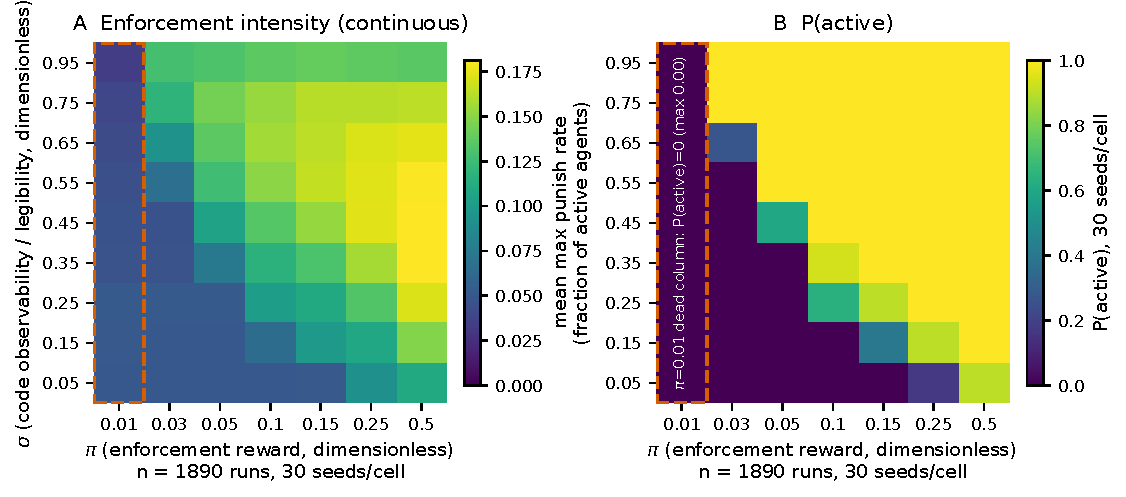
\includegraphics[width=\textwidth]{../figures/manuscript_v2/fig1_activation_frontier.pdf}
\caption{\textbf{Activation frontier under open exit.} Agent-based sweep at $\delta_0=0$ (exit open), $n=1890$ runs (9 $\sigma$ $\times$ 7 $\pi$ cells $\times$ 30 seeds per cell). (A) Mean maximum punish rate, the continuous enforcement-intensity surface. (B) Probability that a run is classified active, recomputed with the hierarchical classifier (active: max punish rate $\geq$ 0.1); overall P(active) $=$ 0.598. Enforcement activates only above a joint $\sigma$--$\pi$ threshold: the $\pi=0.01$ column (dashed outline) is dead in every one of its 9 cells, so an enforcement reward below that level cannot sustain an enforcement apparatus at any level of code observability.}
\label{fig:activation}
\end{figure}

\begin{figure}[htbp]
\centering
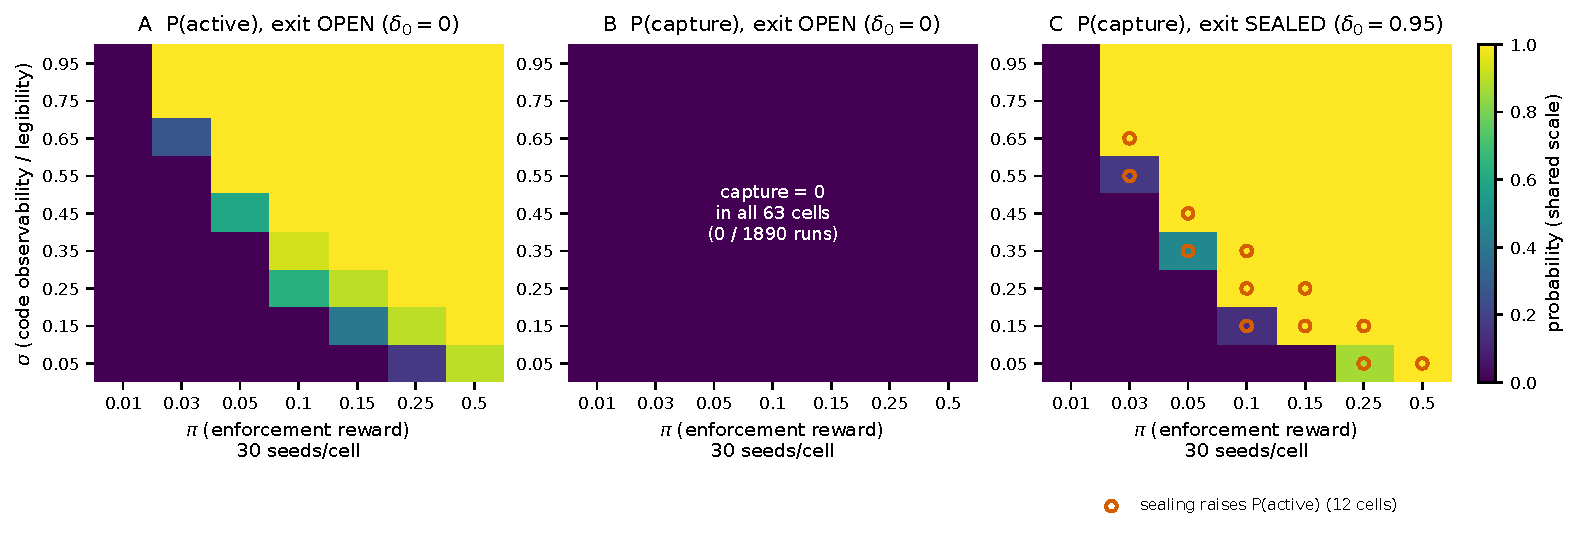
\includegraphics[width=\textwidth]{../figures/manuscript_v2/fig2_two_dimensions.pdf}
\caption{\textbf{Exit closure is necessary for capture.} All panels share one colour scale; 9 $\sigma$ $\times$ 7 $\pi$ cells $\times$ 30 seeds per cell. (A) Probability a run is active with the exit open ($\delta_0=0$, $n=1890$ runs): code geometry alone sets activation, overall P(active) $=$ 0.598. (B) Probability of capture in those same 1890 runs: \textbf{0 of 1890 runs reach capture with the exit open}, in every one of the 63 cells, despite that active rate of 0.598 -- an active enforcement apparatus never converts to capture while members can leave. (C) Probability of capture with the exit sealed ($\delta_0=0.95$, $n=1890$ runs): the same active region now captures. Panels B and C are the same quantity under the two exit conditions, so the contrast isolates the effect of closing the exit. The two dimensions are not fully orthogonal: circled cells in (C) are the 12 of 63 cells where sealing also raises P(active) (mean shift over all cells +0.062; +0.328 among circled cells), and activation falls in no cell. Regimes recomputed with the hierarchical classifier.}
\label{fig:twodim}
\end{figure}

\begin{figure}[htbp]
\centering
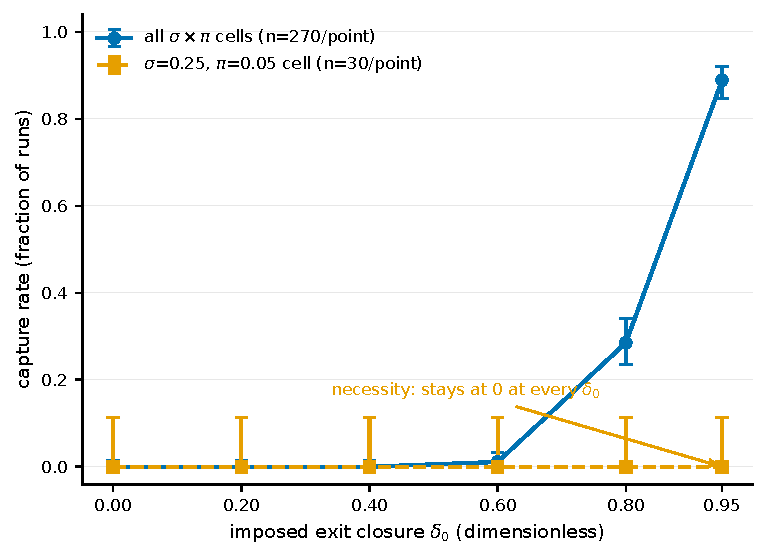
\includegraphics[width=\textwidth]{../figures/manuscript_v2/fig3_exit_closure_dose_response.pdf}
\caption{\textbf{Exit-closure dose-response and the necessity of code geometry.} Capture rate against imposed exit closure $\delta_0$ ($n=1620$ runs total; 270 runs per pooled point, 30 per cell-specific point), with Wilson 95\% intervals. Pooled over all $\sigma\times\pi$ cells (circles) capture rises monotonically from 0.000 at $\delta_0=0$ to 0.889 at $\delta_0=0.95$. In the $\sigma=0.25$, $\pi=0.05$ cell (squares, dashed) the capture rate is 0.000 at every level including $\delta_0=0.95$: closing the exit cannot manufacture capture where the code geometry does not activate. Regimes recomputed with the hierarchical classifier.}
\label{fig:doseresponse}
\end{figure}

\begin{figure}[htbp]
\centering
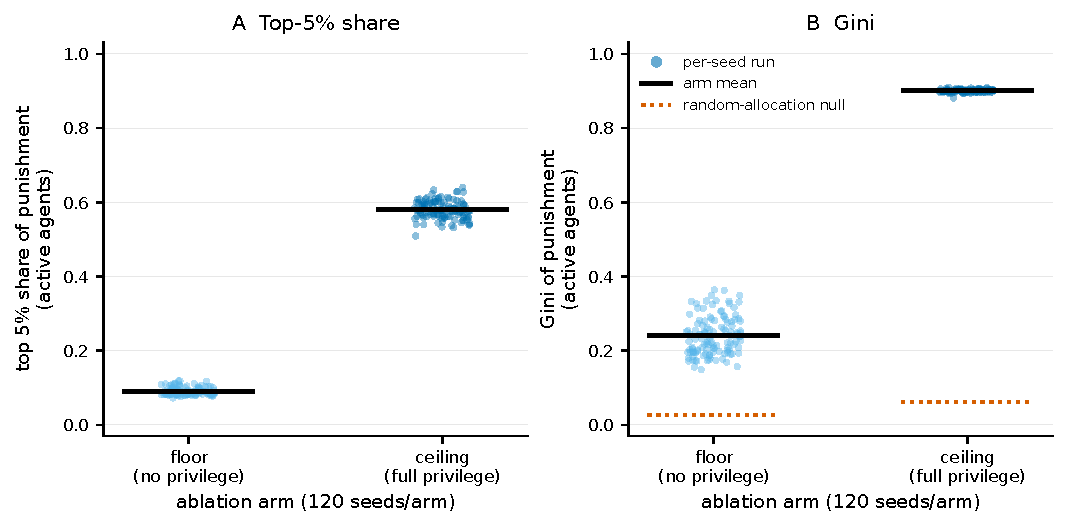
\includegraphics[width=\textwidth]{../figures/manuscript_v2/fig4_privilege_ablation.pdf}
\caption{\textbf{Concentration is manufactured by the privilege architecture.} Role-independent concentration for the ablation floor (no privilege) and ceiling (full privilege bundle), 120 seeds per arm ($n=240$ runs); points are individual runs, black bars arm means. (A) Top-5\% share of punishment among active agents rises from 0.091 at the floor to 0.580 at the ceiling, so 84\% of ceiling concentration is privilege-manufactured. (B) Gini rises from 0.240 to 0.901 against random-allocation nulls (dotted) of 0.028 and 0.062; the floor sits close to its null, so concentration is not an emergent property of the unprivileged model. A committed random-allocation null exists only for the Gini statistic, so panel A carries no null reference.}
\label{fig:ablation}
\end{figure}

\begin{figure}[htbp]
\centering
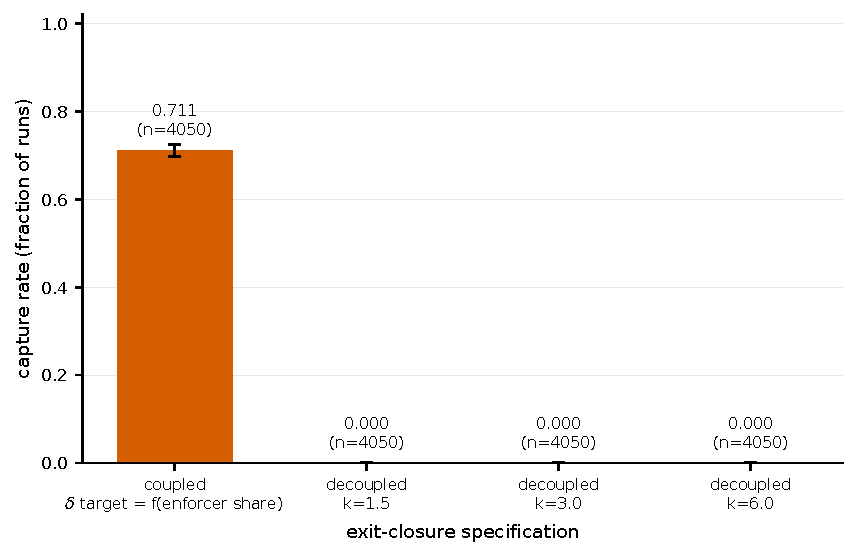
\includegraphics[width=\textwidth]{../figures/manuscript_v2/fig5_circularity_demonstration.pdf}
\caption{\textbf{Capture under the coupled specification is partly definitional.} Capture rate under the coupled exit-closure specification ($n=4050$ runs) versus three decoupled arms ($n=4050$ runs each), Wilson 95\% intervals, regimes recomputed with the hierarchical classifier. The coupled specification sets the exit-closure target as a function of enforcer share ($\delta_{target} = \min(1, \delta_{baseline} + $ enforcer share$)$), an enforcement-concentration quantity, which mechanically drives the retention component of the capture criterion; it yields a capture rate of 0.711. When the closure target is decoupled from enforcer share and driven by punishment intensity instead, the capture rate is 0.000, 0.000 and 0.000 at $k=1.5$, $3.0$ and $6.0$. The contrast shows that the coupled result is produced by the feedback specification rather than by an independent dynamical mechanism.}
\label{fig:circularity}
\end{figure}

\section*{Acknowledgments}

% ============================================================
% REFERENCES
% ============================================================

\begin{thebibliography}{46}

\bibitem{almond2003}
Almond GA, Appleby RS, Sivan E.
\textit{Strong Religion: The Rise of Fundamentalisms around the World}.
University of Chicago Press; 2003.

\bibitem{axelrod1986}
Axelrod R.
An evolutionary approach to norms.
\textit{American Political Science Review}. 1986;80(4):1095--1111.

\bibitem{berman2000}
Berman E.
Sect, subsidy, and sacrifice: An economist's view of ultra-Orthodox Jews.
\textit{Quarterly Journal of Economics}. 2000;115(3):905--953.

\bibitem{berman2008}
Berman E, Laitin DD.
Religion, terrorism and public goods: Testing the club model.
\textit{Journal of Public Economics}. 2008;92(10--11):1942--1967.

\bibitem{boyd2003}
Boyd R, Gintis H, Bowles S, Richerson PJ.
The evolution of altruistic punishment.
\textit{Proceedings of the National Academy of Sciences}. 2003;100(6):3531--3535.

\bibitem{bromley1998}
Bromley DG.
\textit{The Politics of Religious Apostasy: The Role of Apostates in the Transformation of Religious Movements}.
Praeger; 1998.

\bibitem{carvalho2013}
Carvalho JP.
Veiling.
\textit{Quarterly Journal of Economics}. 2013;128(1):337--370.

\bibitem{centola2005}
Centola D, Willer R, Latan\'{e} B.
The emperor's dilemma: A computational model of self-enforcing norms.
\textit{American Journal of Sociology}. 2005;110(4):1009--1040.

\bibitem{cohen2001}
Cohen AB, Rozin P.
Religion and the morality of mentality.
\textit{Journal of Personality and Social Psychology}. 2001;81(4):697--710.

\bibitem{cook2000}
Cook M.
\textit{Commanding Right and Forbidding Wrong in Islamic Thought}.
Cambridge University Press; 2000.

\bibitem{cragun2011}
Cragun RT, Hammer JH.
One person's apostate is another person's convert: What terminology tells us about pro-religious hegemony in the sociology of religion.
\textit{Humanity \& Society}. 2011;35(1--2):149--175.

\bibitem{fehr2000}
Fehr E, G\"{a}chter S.
Cooperation and punishment in public goods experiments.
\textit{American Economic Review}. 2000;90(4):980--994.

\bibitem{fehr2002}
Fehr E, G\"{a}chter S.
Altruistic punishment in humans.
\textit{Nature}. 2002;415(6868):137--140.

\bibitem{fitzpatrick2005}
Fitzpatrick S.
\textit{Tear Off the Masks! Identity and Imposture in Twentieth-Century Russia}.
Princeton University Press; 2005.

\bibitem{fox2019}
Fox J.
The Religion and State Project, Round 3.
Association of Religion Data Archives; 2019.

\bibitem{gelfand2011}
Gelfand MJ, et~al.
Differences between tight and loose cultures: A 33-nation study.
\textit{Science}. 2011;332(6033):1100--1104.

\bibitem{given1997}
Given JB.
\textit{Inquisition and Medieval Society: Power, Discipline, and Resistance in Languedoc}.
Cornell University Press; 1997.

\bibitem{greif2006}
Greif A.
\textit{Institutions and the Path to the Modern Economy: Lessons from Medieval Trade}.
Cambridge University Press; 2006.

\bibitem{greif2016}
Greif A, Mokyr J.
Cognitive rules, institutions, and economic growth: Douglass North and beyond.
\textit{Journal of Institutional Economics}. 2016;13(1):25--52.

\bibitem{hilbe2014}
Hilbe C, Traulsen A, R\"{o}hl T, Milinski M.
Democratic decisions establish stable authorities that overcome the paradox of second-order punishment.
\textit{Proceedings of the National Academy of Sciences}. 2014;111(2):752--756.

\bibitem{hirschman1970}
Hirschman AO.
\textit{Exit, Voice, and Loyalty: Responses to Decline in Firms, Organizations, and States}.
Harvard University Press; 1970.

\bibitem{hagberg2008}
Hagberg AA, Schult DA, Swart PJ.
Exploring network structure, dynamics, and function using NetworkX.
In: \textit{Proceedings of the 7th Python in Science Conference}; 2008. p.~11--15.

\bibitem{iannaccone1992}
Iannaccone LR.
Sacrifice and stigma: Reducing free-riding in cults, communes, and other collectives.
\textit{Journal of Political Economy}. 1992;100(2):271--291.

\bibitem{iannaccone1994}
Iannaccone LR.
Why strict churches are strong.
\textit{American Journal of Sociology}. 1994;99(5):1180--1211.

\bibitem{kelly1989}
Kelly HA.
Inquisition and the prosecution of heresy: Misconceptions and abuses.
\textit{Church History}. 1989;58(4):439--451.

\bibitem{kazil2020}
Kazil J, Masad D, Crooks A.
Utilizing Python for agent-based modeling: The Mesa framework.
In: \textit{Social, Cultural, and Behavioral Modeling}. Springer; 2020. p.~308--317.

\bibitem{kotkin1995}
Kotkin S.
\textit{Magnetic Mountain: Stalinism as a Civilization}.
University of California Press; 1995.

\bibitem{kuran1995}
Kuran T.
\textit{Private Truths, Public Lies: The Social Consequences of Preference Falsification}.
Harvard University Press; 1995.

\bibitem{mann1986}
Mann M.
\textit{The Sources of Social Power, Vol.~1}.
Cambridge University Press; 1986.

\bibitem{norenzayan2013}
Norenzayan A, Gervais WM.
The origins of religious disbelief.
\textit{Trends in Cognitive Sciences}. 2013;17(1):20--25.

\bibitem{north1990}
North DC.
\textit{Institutions, Institutional Change and Economic Performance}.
Cambridge University Press; 1990.

\bibitem{pierson2000}
Pierson P.
Increasing returns, path dependence, and the study of politics.
\textit{American Political Science Review}. 2000;94(2):251--267.

\bibitem{qutb1964}
Qutb S.
\textit{Milestones [Ma'alim fi al-Tariq]}.
Various editions; 1964.

\bibitem{reinhard1983}
Reinhard W.
Zwang zur Konfessionalisierung? Prolegomena zu einer Theorie des konfessionellen Zeitalters.
\textit{Zeitschrift f\"{u}r historische Forschung}. 1983;10(3):257--277.

\bibitem{rubin2017}
Rubin J.
\textit{Rulers, Religion, and Riches: Why the West Got Rich and the Middle East Did Not}.
Cambridge University Press; 2017.

\bibitem{schilling1988}
Schilling H.
Die Konfessionalisierung im Reich: Religi\"{o}ser und gesellschaftlicher Wandel in Deutschland zwischen 1555 und 1620.
\textit{Historische Zeitschrift}. 1988;246(1):1--45.

\bibitem{scott1998}
Scott JC.
\textit{Seeing Like a State: How Certain Schemes to Improve the Human Condition Have Failed}.
Yale University Press; 1998.

\bibitem{sigmund2010}
Sigmund K, De~Silva H, Traulsen A, Hauert C.
Social learning promotes institutions for governing the commons.
\textit{Nature}. 2010;466(7308):861--863.

\bibitem{streib2009}
Streib H, Hood RW, Keller B, Cs\"{o}ff RM, Silver CF.
\textit{Deconversion: Qualitative and Quantitative Results from Cross-Cultural Research in Germany and the United States of America}.
Vandenhoeck \& Ruprecht; 2009.

\bibitem{taleb2018}
Taleb NN.
\textit{Skin in the Game: Hidden Asymmetries in Daily Life}.
Random House; 2018.

\bibitem{tilly1985}
Tilly C.
War making and state making as organized crime.
In: Evans P, Rueschemeyer D, Skocpol T, editors.
\textit{Bringing the State Back In}.
Cambridge University Press; 1985. p.~169--191.

\bibitem{ulmer2008}
Ulmer JT, Bader C, Gault M.
Do moral communities play a role in criminal sentencing? Evidence from Pennsylvania.
\textit{Sociological Quarterly}. 2008;49(4):737--768.

\bibitem{wedeen1999}
Wedeen L.
\textit{Ambiguities of Domination: Politics, Rhetoric, and Symbols in Contemporary Syria}.
Cambridge University Press; 1999.

\bibitem{watts1998}
Watts DJ, Strogatz SH.
Collective dynamics of `small-world' networks.
\textit{Nature}. 1998;393(6684):440--442.

\bibitem{weber1946}
Weber M.
Politics as a Vocation.
In: Gerth HH, Mills CW, editors.
\textit{From Max Weber: Essays in Sociology}.
Oxford University Press; 1946. p.~77--128.
(Original work published 1919.)

\bibitem{yurchak2005}
Yurchak A.
\textit{Everything Was Forever, Until It Was No More: The Last Soviet Generation}.
Princeton University Press; 2005.

\end{thebibliography}

\section*{Data and Code Availability}

All simulation code, data, and analysis scripts are publicly available: an anonymized review copy of the repository is available at [ANONYMOUS-LINK]; the public archive will be linked upon acceptance.

The cross-national regression dataset is provided at \texttt{data/cross\_national\_data.csv}
in the repository.

\section*{Supporting Information}

\noindent\textbf{Online Resource 1.} Scoring rubric anchors (0--4 scale definitions for all five code-geometry dimensions), complete parameter tables, illustrative regime scores with source citations, regime classification threshold sensitivity ($\pm$5 pp), monopoly ablation results (180 runs), cadre quota sensitivity (180 runs), intensity gate sensitivity (180 runs), bootstrap regression analysis (10,000 resamples), and drift mechanism technical details.

\end{document}
